
%%%%%%%%%%%%%%%
%%%      CHAPTER      %%%
%%%%%%%%%%%%%%%

\chapternonum{Foreword}
\label{ch:general_introduction:foreword}
\addcontentsline{toc}{chapter}{Foreword}

I precisely remember the first book of theoretical biology I read. At this time, I was an aircraft mechanic, apparently far from the academic world. With \textit{Chance and Necessity}, Jacques Monod made a remarkable demonstration of the central dogma of molecular biology, introduced 12 years ago by Francis Crick \citep{crick-1958}. As a novice, I have been impressed by the clarity and the rigor of this philosophical essay, stamped with a certain arrogance to have explained everything about life on Earth.

\begin{quote}
L'ultima ratio de toutes les structures t\'{e}l\'{e}onomiques des \^{e}tres vivants est donc enferm\'{e}e dans les s\'{e}quences de radicaux des fibres polypeptidiques, ``embryons'' de ces d\'{e}mons de Maxwell biologiques que sont les prot\'{e}ines globulaires. En un sens, tr\`es r\'{e}el, c'est \`a ce niveau d'organisation chimique que g\^{i}t, s'il y en a un, le secret de la vie. Et saurait-on non seulement d\'{e}crire ces s\'{e}quences, mais \'{e}noncer la loi d'assemblage \`a laquelle elles ob\'{e}issent, on pourrait dire que le secret de la vie est perc\'{e}, l'ultima ratio d\'{e}couverte \citep{monod-1970}.
\end{quote}

This book sowed the seeds of my fascination for evolutionary biology.
In the following year, I went back to school with this kind of convictions: living organisms own a ``genetic program'', encoding for their phenotype.
This program is regularly altered by purely random mutations, thereby providing the fuel for evolution. I found comfortable consistency with this dogma in the first lessons I followed at university. The apotheosis has probably been reached on reading \textit{The Selfish Gene} by Richard Dawkins \citep{dawkins-1976}.

During my first year of college, I met astonishing people\footnote{See the acknowledgments.} that pushed me to take a more measured look at theoretical biology. In particular, I had the opportunity to read the work of Jean-Jacques Kupiec \citep{kupiec-2000,kupiec-2008}, a fervent partisan of nominalism in science, that definitively influenced my scientific itinerary. While J-J. Kupiec's narrative is tinged with a touch of bitterness, his epistemology has the merit to promote thought and criticism. I will always remember the little joke I heard at the time: ``\textit{People believing that stochastic gene expression is important are often to the left, people believing that a genetic program exists are often to the right}''\footnote{A classical debate between essentialist and nominalist views in sum.}. 

Armed with this very small, but necessary epistemological knowledge, I finally read \textit{On the Origin of Species} by Charles Darwin. I was not surprised to discover that his reasoning was almost at the opposite from Jacques Monod's ones. While the latter stated that the three properties distinguishing living organisms from the rest of the universe were teleonomy, autonomous morphogenesis and reproductive invariance, Charles Darwin original theory defined individual differences and natural selection as the main properties of life.

\begin{quote}
No one supposes that all the individuals of the same species are cast in the very same mould. These individual differences are highly important for us, as they afford materials for natural selection to accumulate, in the same manner as man can accumulate in any given direction individual differences in his domesticated productions \citep{darwin-1859}.
\end{quote}

Indeed, a form of essentialism flowed back in biology in the 1960's, mainly following Erwin Schr\"odinger's book \textit{What is Life?} \citep{schrodinger-1944}, and the discover of DNA structure \citep{avery-et-al-1944,watson-et-al-1953}. According to E. Schr\"odinger, most physical properties on a large scale (\textit{e.g.} diffusion process or kinetic theory of gases) emerge from chaos at a low scale: this property is known as the principle of order-from-disorder. On the contrary, living matter ``\textit{is likely to involve `other laws of physics' hitherto unknown, which however, once they have been revealed, will form just as integral a part of science as the former}'' \citep{schrodinger-1944}. E. Schr\"odinger was believing in a principle of order-from-order, the living matter escaping from thermodynamics laws. This point of view, while probably never accepted as is by convinced darwinists\footnote{In \textit{Chance and Necessity}, J. Monod largely argued against the principle of order-from-order in life. However, all the paradox of his interpretation of life resurged when he used the term ``Maxwell's demons'' to design enzymes.}, still influences nowadays scientific works.

\begin{quote}
Pour la biologie mol\'{e}culaire, l'organisme est donc toujours une machine d\'{e}terministe, mais la vieille horloge de Descartes a \'{e}t\'{e} remplac\'{e}e par un ordinateur \citep{kupiec-2008}.
\end{quote}

As a consequence, a paradoxical representation of life pervaded theoretical biology for decades: while a small ``Copernican revolution'' was accomplished in evolutionary biology with C. Darwin, a strong essentialism was hidden in the wood, particularly in molecular biology.

One example is the strong belief that genes are the fundamental units of natural selection. Initially, genes have been defined as inheritable units predetermining\footnote{One could ask why a causation was introduced, while just a correlation was observed.} phenotypic traits \citep{johannsen-1911} (W. Johannsen also introduced the notions of genotype and phenotype). As discussed right above, the discover of DNA and the mechanisms of gene expression reinforced this view and led to a ``genocentric'' view of evolution, with a clear separation between the genotype, undergoing mutations and inherited, and the phenotype \citep{rivoire-and-leibler-2014}. This net separation is often criticized as a resurgence of an Aristotelian interpretation of life\footnote{The model (the essence) of an organism is encoded in its genotype, out of the scope of natural selection (in the world of ideas), its phenotype being an imperfect instantiation of the model (in the sensible world).}, against the evident nominalism of C. Darwin. \textit{The selfish gene} by \cite{dawkins-1976} is often cited as a culmination of genetic reductionism in biology.

Another consequence of essentialism in biology is the belief that mutations purely occur at random. As stated by \cite{monod-1970}, the purpose---or teleonomy---of any living organism is to transmit its intact genotype---by reproductive invariance---to its offspring. Of course, as explained by J. Monod himself, teleonomy is not teleology: the apparent finalism of life is a consequence of natural selection. But the damage is done: in the face of teleonomy and reproductive invariance, the way mutations occur is necessarily out of the scope of selection. For decades, any statement that organisms could partly control the way mutations occur (\textit{e.g.}, the evolution of mutation rates, globally or locally on the genome), was accused of finalism---which is indeed quite paradoxical. In the last decades, this dogmatic view has been undermined by experimental an theoretical highlights, leading to the idea that evolution could shape its own fate. This phenomenon is usually known as the evolution of evolvability.

A last example I would give is the classical interpretation of organismal development as a genetic program, deterministically expressing the phenotype from the genotype:
``\textit{chaque \oe uf contient donc, dans les chromosomes re\c cus de ses parents, tout son propre avenir, les \'etapes de son d\'eveloppement, la forme et les propri\'et\'es de l'\^etre qui en \'emergera. L'organisme devient ainsi la r\'ealisation d'un programme prescrit par l'h\'er\'edit\'e}'' \citep{jacob-1970}\footnote{These words could remind the preformationist views developed during the XVII\textsuperscript{th} century.}.
An essential role is attributed to the concept of protein stereospecificity, conferring to the cell the ability to run deterministic and logical tasks based on signaling and regulation pathways. As stated by \cite{kupiec-2008}: ``\textit{bien que cela soul\`eve de nombreux probl\`emes, ce programme g\'{e}n\'{e}tique a \'{e}t\'{e} con\c cu par analogie avec un programme informatique}''. However, biochemical reactions do not escape thermodynamics laws, and the low number of molecules involved in many biological processes implies that ``\textit{chance is at the heart of the cell}'' \citep{gandrillon-et-al-2012}. Nowadays, the stochastic nature of cellular functioning is widely documented and accepted, but its consequences on the evolution of biological organisms are still largely unknown.

Of course, there is no sense to criticize \textit{a posteriori} the work of an entire scientific community, without considering the extraordinary progresses of biology during the XX\textsuperscript{th} century.
This is why my thesis work will be mostly based on the rationale that the tools and models of theoretical evolutionary biology proven to be efficient can be revisited, extended or modified to ask new scientific questions.

The starting point of my thesis work is the process of evolution of evolution, or EvoEvo, as coined by \cite{hindre-et-al-2012}, that encompasses the evolution of variability, evolvability, robustness and open-endeness.

There is no scientific theory without modeling \citep{servedio-et-al-2014}. I explored two different---but not opposite---modeling approaches to study EvoEvo: mathematical modeling and multi-scale individual-based simulations. On this particular point, I have been strongly influenced all along my stay in the INRIA-Beagle team by the complementary approach of Carole Knibbe and Guillaume Beslon, well-resumed by the quadruplet ``\textit{Create, Play, Experiment, Discover}'', used as a slogan for the 14\textsuperscript{th} European Conference on Artificial Life.

As explained in chapter \ref{ch:general_introduction:introduction}, there is a deep sense to tackle EvoEvo by these two modeling sides. The first, and most obvious reason is that analytical demonstrations are needed to sit a theory and convince a scientific community. The second reason is more specific to EvoEvo: the evolution of an organism implies the interaction of many biological organization levels, with different temporalities and scales. To properly understand how evolution shapes such a complex system, we need to simulate it with a multi-scale model catching, at least partially, this complexity \citep{lavelle-et-al-2008}. As stated by S. L. Peck: ``\textit{The world is complex and we need all the tools that we can muster to understand it}'' \citep{peck-2004}.

This manuscript is structured as following: in a first chapter, I will introduce the concept of evolution of evolution, and the modeling approaches used to decipher some of its aspects. Then, in part \ref{part1}, I will present a mathematical modeling study on the evolution of phenotypic noise. This model extends Fisher's geometric model \citep{fisher-1930}. In part \ref{part2}, I will introduce {\EvoEvoSim}, a multi-scale model of \textit{in silico} experimental evolution \citep{hindre-et-al-2012} dedicated to the study of evolution of evolution (chapter \ref{ch:part2:methodology}). Two results obtained with this model will be presented, one on niche construction and the evolution of stable cross-feeding (chapter \ref{ch:part2:first_result}), another on the evolution of regulation when organisms undergo strong energy trade-offs (chapter \ref{ch:part2:second_result}).

Some of these results have been published, or submitted to scientific journals. Others come from documents produced in the course of the FP7 EvoEvo project I were involved in, or are preliminary. I will indicate it when it will be the case. This manuscript also contains appendices; I will refer to them in the main text when necessary.

\newpage

\begin{quote}
Some rain forests in the Amazon region occur on white-sand soils. In these locations, the physical environment consists of clean white sand, air, falling water, and sunlight. Embedded within this relatively simple physical context, we find one of the most complex ecosystems on earth, containing hundreds of thousands of species. These species do not represent hundreds of thousands of adaptations to the physical environment. Most of adaptations of these species are to the other living organisms. The forest creates its own environment. \citep{ray-1993}
\end{quote}

\begin{figure}[!h]
\centering
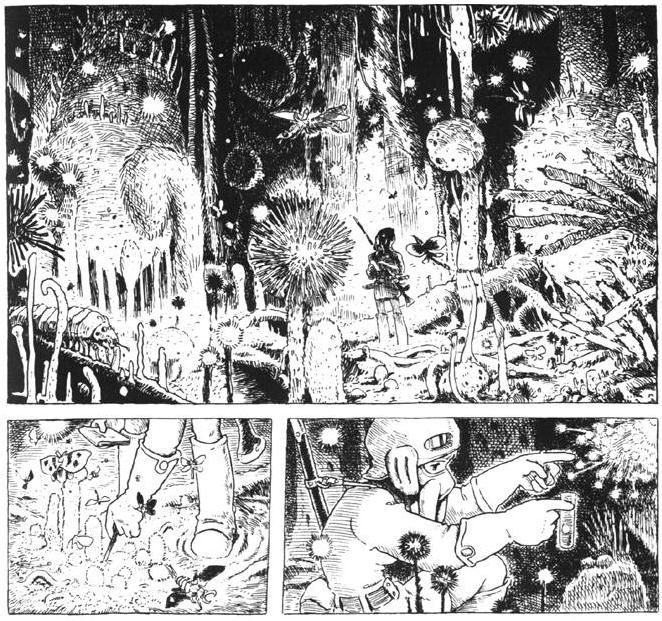
\includegraphics[width=0.8\textwidth]{nausicaa.jpeg}
\caption[An example of complex ecosystem.]{{\bf An example of complex ecosystem.} From \textit{Nausica\"a}, by Hayao Miyazaki.}
\label{fig:nausicaa}
\end{figure}

